\documentclass[licentiate,utf8,lot,loar,lof,shortloft,index]{jydiss}
%\documentclass[licentiate,latin9,loa,lot,lof,shortloft,captiondot]{jydiss}
%\documentclass[licentiate,finnish,latin9,loa,lot,lof]{jydiss}
\usepackage{algorithm}% http://ctan.org/pkg/algorithms
\usepackage{algpseudocode}% http://ctan.org/pkg/algorithmicx
\usepackage{listings}
\usepackage{hyperref}
\usepackage{enumitem}
\usepackage{array}
\usepackage{amsmath}
\usepackage{amssymb}
\usepackage{tikz,ulem}
\usepackage{graphics}
\usepackage{standalone}
\usepackage{amsthm}
\usepackage{breakcites}

%\usepackage{ltexpprt}
%\algtext*{EndWhile}% Remove "end while" text
%\algtext*{EndIf}% Remove "end if" text
%\algtext*{EndFor}% Remove "end if" text
\usepackage{cite}
%\usepackage{graphicx}
\usepackage{soul} % to cross text
\usepackage{enumitem}




\newtheorem{definition}{Definition}
\newtheorem{theorem}{Theorem}

\newcommand*{\LargeCdot}{\raisebox{-0.5ex}{\scalebox{1.8}{$\cdot$}}}
\newlist{WithAxioms}{enumerate}{1}
\setlist[WithAxioms]{label=Axiom \arabic*:}


\newcommand{\T}{\mathcal{T}} % index set
\newcommand{\Collect}[1]{\langle #1 \rangle} % vector/sequence notation
%\newcommand{\Ed}[1]{\colorbox{green!20}{#1}} % highlight editions
\newcommand{\Ed}[1]{{\color{blue!100}#1}} % highlight editions
\newcommand{\Eq}[1]{Eq.(\ref{#1})} % ref equations as Eq.(reference)
\newcommand{\lbl}[1]{(#1)} % to denote output labels of classifier
%\newcommand{\Event}[2]{\mathtt{E}(#1)^{#2}} % to denote CdEs (+ or -)
%\newcommand{\Event}[2]{\mathbf{e}(#1)^{#2}} % to denote CdEs (+ or -)
\newcommand{\Event}[2]{\mathbf{e}_{#1}^{#2}} % to denote CdEs (+ or -)


% from blpa 
\def \BD   {\textbf{BD }}
\def \PCCF {\textbf{PCCF }} 
\def \PCCFWithoutSpace {\textbf{PCCF}} 
\def \LEAP {\textbf{LEAP }} 

%\newcommand{\Collect}[1]{\langle #1 \rangle} % vector/sequence notation
%\newcommand{\Event}[2]{\mathbf{e}_{#1}^{#2}} % to denote CdEs (+ or -)
%\newcommand{\lbl}[1]{(#1)} % to denote output labels of classifier
%\newcommand{\T}{\mathcal{T}} % index set
%\newcommand{\Eq}[1]{Eq.(\ref{#1})}

\newcommand{\GammaDistr}{\text{Gamma}}

\DeclareMathOperator*{\argmax}{\argmax}

\newcommand{\PccfII}[2]{\textit{Pccf}(#1,#2)}
\newcommand{\PccfI}[1]{\textit{Pccf}(#1)}

%\newcommand*{\LargeCdot}{\raisebox{-0.5ex}{\scalebox{1.8}{$\cdot$}}}

\def\mucommon        {\tilde{\mu}}
\def\muzerocommon    {\tilde{\mu}_0}
\def\sigmacommon     {\tilde{\sigma}}
\def\xcommon         {\tilde{x}_i}
\def\taucommon       {\tilde{\tau}}
\def\kappazerocommon {\tilde{\kappa}_0}
\def\kappacommon     {\tilde{\kappa}}
\def\alphazerocommon {\tilde{\alpha}_0}
\def\alphacommon     {\tilde{\alpha}}
\def\betazerocommon  {\tilde{\beta}_0}
\def\betacommon      {\tilde{\beta}}


\title{Predictive analytics with online changedetection in data streams}
% \entitle{foo}
\setauthor{\rm Alexandr}{\rm Maslov}

%----------------------------------------------------------------------------------%
\abstract{
    This is an English abstract.
}
%----------------------------------------------------------------------------------%

\keywords{
  Change detection, 
  error correction, \\
}

\people{
\item[Author]
  \textit{Alexandr Maslov} \\
    Department of Mathematics and Computer Science\\
    Eindhoven University of Technology (TU/e) \\
    and\\
    Department of Mathematical Information Technology\\
    University of Jyv\"{a}skyl\"{a} (JYU)\\
    Finland

    \item[Supervisors] 
      \textit{Prof. Dr. Mykola Pechenizkiy}\\[0.3em]
      Department of Computer Science\\
      Department of Computer Science\\
      Eindhoven University of Technology (TU/e)\\
      The Netherlands\\

      \textit{Prof. Dr. Tommi K\"{a}rkk\"{a}inen}\\[0.3em]
      Department of Mathematical Information Technology\\
      University of Jyv\"{a}skyl\"{a}\\
      Finland

    \item[Reviewers] XXX
    XXX
%	\item[Reviewers] 
%		
%		\textit{Prof. Dr. Roland Glowinski}\\[0.3em]
%		University of Houston \\
%		Department of Mathematics \\
%		Houston, TX \\
%		USA
%		
%		\textit{Prof. Dr. Ulrich Langer}\\[0.3em]
%		Institute of Computational Mathematics \\
%		Johann Radon Institute for Computational and \\
%		Applied Mathematics (RICAM) \\
%		Austrian Academy of Sciences (\"{O}AW) \\
%		Austria
    % \item[Opponent] XXX
}
\isbn[nid.]{123-456-78-9012-3}
\isbn[PDF]{345-678-90-1234-5}
%\makeindex
% Tommi K\"{a}rkk\"{a}inen
%        \email{tommi.karkkainen@jyu.fi}
%       \affaddr{Dept. of Mathematical IT,}\\
%       \affaddr{University of Jyv\"{a}skyl\"{a}}\\
%       \affaddr{P.O. Box 35, FIN-40014}\\
%       \affaddr{Finland}\\
%       \email{tommi.karkkainen@jyu.fi}
% Mykola Pechenizkiy
%        \affaddr{Dept. of CS, TU Eindhoven}\\
%\affaddr{P.O. Box 513, NL-5600MB}\\
%\affaddr{the Netherlands}\\
%\email{a.maslov@tue.nl,\\ m.pechenizkiy@tue.nl}
%%%%%..... END JYU TEMPLATE



\makeindex
\begin{document}

\preface

\index{aaaaa} aaaaa

\acknowledgements

\begin{notations}
\notation{$:=$}{equals by definition}
\end{notations}

\mainmatter

%===============================================================================%
%                              INTRODUCTION 
%===============================================================================%
\chapter{Introduction}
In the real world, data distributions are almost never static.


\chapter{Concept drift problem}
%===============================================================================%
Concept drift~\cite{schlimmer1986incremental,gama2014survey} is a
phenomenon when relation between the input data and the target variable changes
over time~\cite{gama2014survey}.
Formally can be defined~\cite{gama2014survey} as Equation\ref{eq:concept_drift} 
\begin{equation}\label{eq:concept_drift}
\exists X: p_{t_0}(X,y) \neq  p_{t_1}(X,y)
\end{equation}
Adaptive learning refers to updating model online to react to concept
drifts~\cite{gama2014survey}.
%===============================================================================%
\chapter{Change detection problem}
Machine Learning models learn the relation between input data $X$ and target
variable $y$ by approximating a joint distribution $P(X,y)$.  Model performance
degrades when learned underlying data distribution changes.  Therefore concept
drift can be detected by monitoring change points in model's output performance
statistics.
%===============================================================================%
On-line change detection in time series data is an old practical problem with
the roots in the problem of statistical quality
control~\cite{basseville1993detection}, ~\cite{NISTbook}.  Walter A. Shewhart
invented control charts in 1924 while working on the problem of statistical
quality control to improve reliability of telephone transmission systems.
%===============================================================================%
Quality control example: $X$ is a set of sensor readings and $y=good$ is a
quality of the produced item.
%===============================================================================%
Offline and online.
In offline learning all training data is available during training.
In online learning the data is processed sequentially from data streams.
Model is being updated as more data arrives.
Data evolve over time in dynamically changing environments.

\section{Adwin}

\begin{figure}[!htb]
	\centering
	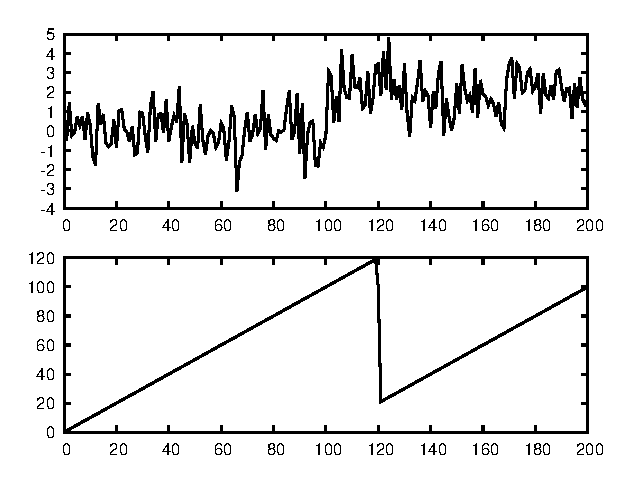
\includegraphics[width=0.9\textwidth]{images/example_output_adwin.eps}
	\caption{ADWIN}\label{fig:adwin_output_example}
\end{figure}

\section{PELT method}
Offline detector used in online settings in ~\cite{marrero2013aclac}.
~\cite{killick2012optimal}
Pelt method is based on a common approach of  minimising a cost function over possible numbers and locations of change points.
Pelt is based on~\cite{jackson2005algorithm}, but involves a pruning step reducing the computational cost but not affecting exactness of the resulting segmentation.
Dynamic programming~\cite{bellman1966dynamic}.

Time interval $I$.
Ordered sequence of data $y_{1:n}=(x_1,\dots,y_n)$.
A partition $P$ of an interval $I$ is a set of blocks is defined  by change points $\tau_{1:m}=(\tau_1, \dots, \tau_m)$.
Each change point is an integer between 1 and $n-1$.
We define $\tau_0=0$ and $\tau_{m+1}=n$.
$m$ change points split the data into $m+1$ segments, $i$-th segment is $y_{\tau_{i-1} : \tau_i}$.
For example, if there is one changepoint $\tau_1$ the segments are $B_1=y_{\tau_0:\tau_1}$ and $B_2=y_{\tau_1:\tau_2}$ where $\tau_2 \equiv n$.
The goal is to find an optimal partition by minimising the cost function defined by Equation\ref{eq:cost_function}
\begin{equation}\label{eq:cost_function}
	\sum_{i=1}^{m+1} [ C(B_i) ] + \beta f(m),\: \text{where } B_i \equiv y_{\tau_{i-1} : \tau_i}
\end{equation}
where $\beta f(m)$ is a regularization term to prevent overfitting.
Commonly used cost functions are twice the negative log likelihood~\cite{guyon1999underfitting,chen2011parametric},
quadratic loss and cumulative sums~\cite{inclan1994use, rigaill2010pruned}. 
The most common choices for the regularization term are usually $\beta f(m) = \beta m$.
Examples are Akaike's Information Criterion (AIC\cite{akaike1974new}) $\beta=2p$ and Schwartz Information Criterion (BIC\cite{schwarz1978estimating}) ($\beta = p \log{n}$) where $p$ is the number of additional parameters introduced by adding a new changepoint.
Dynamic programming optimal segmentation is based on the next principle of optimality
\begin{theorem}
Let $P^{\text{max}}$ be an optimal optimal partition of $I$
\end{theorem}	

\begin{algorithm}[!h]
	\begin{algorithmic}
		\Function{pelt}{$Y$, $\sigma$, $C(s,t)$}
		\State n = length($Y$)
		\State $F$ = zeros(n)\Comment{Optimal segmentation costs till $t$}
		\State $F[0] = - \log(n)$
		\State previous\_changes\_opt = zeros[n]\Comment{Optimal previous change location}
		\For{t $\in$ [2, n]}
		    \State previous\_changes\_possible = $1,\dots,t-1$
		    \State i = 0
		    \For{s $\in$ previous\_changes\_possible}
		         \State i += 1
		        \State segmentation\_costs[i] = $C(s, t)$
		    \EndFor
		    \State costs = $F[\text{previous\_changes\_possible}]$ + segmentation\_costs + $\log(n)$
		    \State $F[t+1] = min(\text{costs})$
		    \State $\text{previous\_changes\_opt}[t] = \text{previous\_changes\_possible}[argmin(\text{costs})]$
		\EndFor
		\State detections = $\text{fn\_extract\_detections(previous\_changes\_opt)}$
		\EndFunction
	\end{algorithmic}
\end{algorithm}

\begin{figure}[!htb]
	\centering
	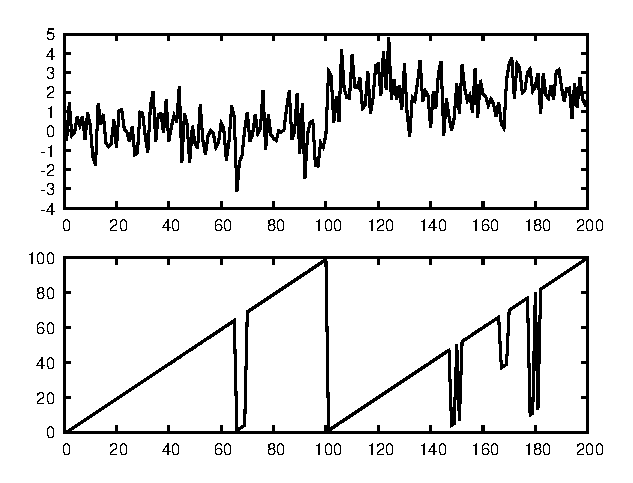
\includegraphics[width=0.9\textwidth]{images/example_output_pelt.eps}
	\caption{PELT}\label{fig:pelt_output_example}
\end{figure}


\section{Bayesian detector}
\cite{adams2007bayesian}
BD detector works by recursively estimating posterior probability distribution $P(r_t | \pmb{x}_{1:t}, \theta)$ of the \textit{run length} variable $r_t$ which is a time since the last changepoint.
Changepoint is an event when
\begin{equation}
	\operatorname*{arg\,max}_{r_t} P(r_t | \pmb{x}_{1:t}, \theta) = 0
\end{equation}
%\[\]
%$r_t = 0$
Every time a new measurement $x_t$ is observed the \textit{posterior} distribution is recalculated using the Bayes` theorem to update parameters of the distributions used to model data
\[
(r_t | \pmb{x}_{1:t}) = \frac{P(r_t, \pmb{x}_{1:t})}{P(\pmb{x}_{1:t})}
\]
and the law of total probability
%$P(x) = \sum_{y} P(x|y) p(y)$
\begin{equation}
	P(r_t|\:\LargeCdot) = \sum_{r_{t-1}} P(r_{t} | \: r_{t-1},\:\LargeCdot) \: P(r_{t-1}|\:\LargeCdot)
\end{equation}
to take into account values from all the runs in the past.
The \textit{prior} probability of the change $P(r_t=0|t)$ in BD detector is specified using the constant-value hazard rate $h$ which is a prior probability to observe a change and which is supposed to be known before the change detection process starts.
\begin{figure}[!htb]
	\centering
	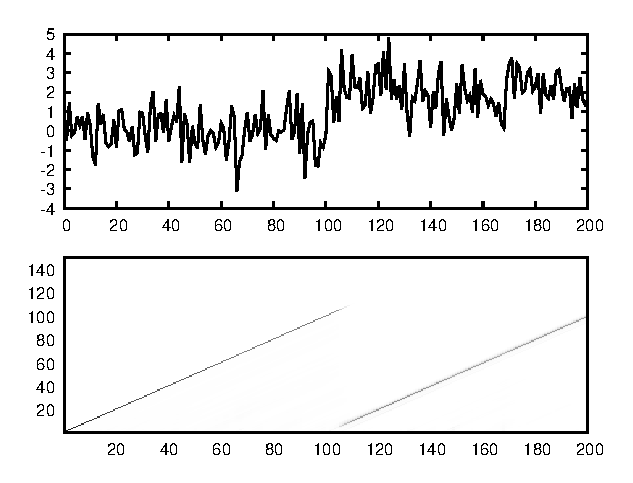
\includegraphics[width=0.9\textwidth]{images/example_output_bayes.eps}
	\caption{Bayes}\label{fig:bayes_output_example}
\end{figure}

\section{CUSUM detector}
In this section, we describe the CuSum~\cite{Page1954} detector and its output statistic properties important for measuring performance metrics in static and dynamic settings.
Changes in the stream of measurements reflect dynamics of observed phenomenon happening in time.
Therefore, strictly speaking, any change is a gradual process.
In this paper, for simplicity, we refer to change points and to detections as individual time moments as if change would have happen instantly. If change is gradual and spans time interval then it can be reduced to a single time moment by considering the start or end of the change event~\footnote{Gradual change may become represented as an abrupt change in the time series also due to the sampling rate of measurements}. 
Change points in the signal are characterized by the time moment when they happened and by the corresponding mean shift value in the signal.
\begin{definition}
	Change point is a time moment $t^c$ when statistical properties of the data stream change significantly accordingly to a predefined criteria.
\end{definition}
\begin{definition}
	Detection is a time moment $t^d$ when a detector alarms a change.
\end{definition}
For example, if $x_i \sim \mathbb{N}(\mu_1, \sigma)$ for $i < k$ and $x_i \sim \mathbb{N}(\mu_2, \sigma)$ for $i \geq k$,
then we say that a change point occurred at time moment $t_k$, i.e. $t^{\text{c}}_{k} \equiv t_k$.
In general, detection can usually be alarmed before or after a change point.
If $t^{\text{d}}_k > t^{\text{c}}_k$, then change is detected with the delay $t^{\text{d}}_k - t^{\text{c}}_k$.
%TOMMI: Can we give definition like below? I.e. to say that ALL too-early alarms are false alarms?
If $t^{\text{d}}_k < t^{\text{c}}_k$ then detection $t^{\text{d}}_k$ is a false alarm (FA).

As an input, CuSum detector receives time series of observations~\ref{eq:input_ts} usually taken at constant sampling rate.
\begin{equation}\label{eq:input_ts}
	(x_i)_{i=1}^{N} \equiv (x_1, x_2, \dots, x_N)
\end{equation}
taken at corresponding time moments $(t_i)_{i=1}^N$.
Observations and time moments are enumerated by index $i$ mapping $t_i$ to observations $x_i$ and vice versa.
CuSum works through a sequential calculation of the output statistic as follows
% Cusum rule: https://www.itl.nist.gov/div898/handbook/pmc/section3/pmc323.htm
\begin{align}
	S_0 &= 0 \nonumber \\
	S_{n} &= \max (0, S_{n-1} + x_n - \mu_0 - k )\label{eq:cusum_scheme}.
\end{align}
% Detections are alarmed at time moments when Cusum's output statistic exceeds a threshold value $h$.
Detections are alarmed at time moments when $S_{t+1} > h$, i.e. when output statistic exceeds a threshold value $h$.
In \eqref{eq:cusum_scheme}, $\mu_0$ is the estimate of the in-control state signals' mean value.
The parameter $k$ is called allowance value and it depends on the level of mean shift $\delta=\mu_2-\mu_1$ that we aim to detect.
\begin{figure}[!htb]
	\centering
	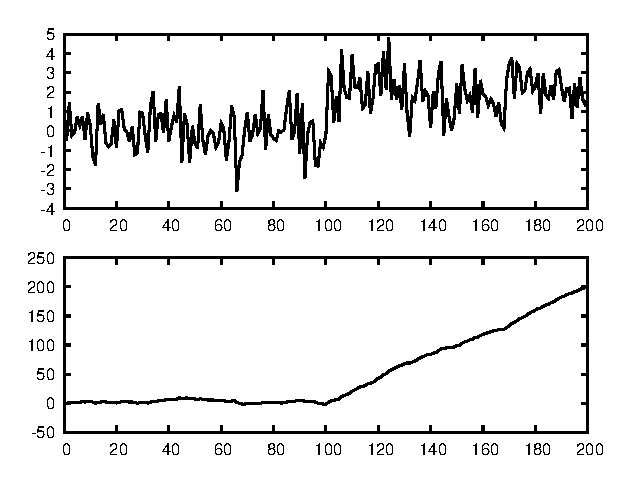
\includegraphics[width=0.9\textwidth]{images/example_output_cusum.eps}
	\caption{CuSum}\label{fig:cusum_output_example}
\end{figure}

%===============================================================================%
%                               RECURRENCY
%===============================================================================%
\chapter{Predictability And Recurrency}
Adaptive learning in concept drift.
Predictability of events in the data stream.
~\cite{feller2008introduction}
Sums of independent random variables.
Recurrency is a form of predictability.

\section{Inter-arrival times modeling}
Commonly used probability distributions for modelling inter-arrival times.


\chapter{Main results}
~\cite{MaslovSDM2016, MaslovIJCNN2017}
\section{Pccf}
\section{Integration with Bayesian detector}
\section{Integration with CuSum}

\chapter{MISC}
External~\cite{shewhart1931economic}
Included article~\cite{sha1}.
Concept drift and change detection problem.
Concept drift can be reduced to change detection in univariate time series?


\begin{itemize}
  \item Change detection:~\cite{basseville1993detection}
  \item Sequential change detection problem is a well studied problem, see for example in~\cite{tartakovsky2014sequential}, ~\cite{plasse2021streaming}. 

  \item Optimality of the change detection procedure was investigated in~\cite{Page1954},~\cite{Shiryaev2010,Shiryaev1961,Shiryaev1963}.
  Asymptotic and nonasymptotic optimality of cumulative sum algorithms was provedin~\cite{lorden1971procedures},~\cite{moustakides1986optimal},~\cite{moustakides2004optimality},~\cite{ritov1990decision}. In~\cite{Shiryaev1963,shiryaev2007optimal} the change point is modelled as a random variable with a known geometric distribution~\cite{veeravalli2014quickest} and optimal algorithm minimizing the average detection delay given constraint on the probability of false alarm is proposed. In our work we minimize the detection delay given a constraint on the maximum delay imposed by the prediction interval width. In~\cite{lorden1971procedures} asymptotic optimality of Cusum~\cite{Page1954} is proved according to the minimax criterion for delay with the mean time between false alarms going to infinity.

  \item Concept drift:
\end{itemize}

\chapter{Conclusion}

\tailmatter
\finnishsummary
Foo bar
%\inputencoding{utf8}
\bibliographystyle{plain}
\bibliography{references}
\appendices
\appendix{A}
\section{foobar}

\backmatter

\includedarticles
\begin{article}{sha1}
	\arttitle{Modelling Recurrent Events for Improving Online Change Detection}
	\artauthor{Alexandr Maslov, Mykola Pechenizkiy, Indr{\.e} {\v{Z}}liobait{\.e}, and Tommi K\"{a}rkk\"{a}inen}
	\artpublish{Proceedings of the 2016 SIAM International Conference on Data Mining}
	\artyear{2016}
	\artcopyright{XX}
	\artpages{1}
\end{article}

\begin{article}{sha2}
	\arthide
	\arttitle{BLPA: Bayesian learn-predict-adjust method for online detection of recurrent changepoints}
	\artauthor{Alexandr  Maslov, Mykola Pechenizkiy, Yulong  Pei, Indre {\v{Z}}liobait{\.e},  Alexander Shklyaev, Tommi Karkk{\"a}inen, and Hollm{\'e}n, Jaakko}
	\artpublish{2017 International Joint Conference on Neural Networks (IJCNN)}
	\artyear{2017}
	\artcopyright{XXX}
\end{article}
\printindex
\end{document}
